\documentclass[english,9pt,aspectraio=169]{beamer}
\usepackage{etex}
\usetheme{uzhneu-en-informal}
%\usepackage{uarial}
\usepackage[T1]{fontenc}
\usepackage[utf8]{inputenc}
\RequirePackage{graphicx,ae}
\usepackage{bm}
\usepackage{fancybox,amssymb,color}
\usepackage{pgfpages}
\usepackage{booktabs}
\usepackage{verbatim}
\usepackage{animate}
\usepackage{numprint}
\usepackage{vwcol} 
\usepackage{dsfont}
\usepackage{tikz}
\usepackage{amsmath,natbib}
\usepackage{mathbbol}
\usepackage{babel}
\usepackage{SweaveSlides}
\usepackage{multicol}
\usepackage{xcolor}


\usetheme{uzhneu-en-informal}
\DeclareMathOperator{\po}{Poisson}
\DeclareMathOperator{\G}{Gamma}
\DeclareMathOperator{\Be}{Beta}
\DeclareMathOperator{\logit}{logit}
\def\n{\mathop{\mathcal N}}

\definecolor{Gray}{RGB}{139,137,137}
\definecolor{darkred}{rgb}{0.8,0,0}
\definecolor{Green}{rgb}{0,0.8,0.3}
\definecolor{lightgreen}{rgb}{0,0.7,0.3}
\definecolor{Blue}{rgb}{0,0,1}
\def\myalert{\textcolor{darkred}}
\def\myref{\textcolor{Gray}}
\setbeamercovered{invisible}

\renewcommand{\baselinestretch}{1.2}
\beamertemplateballitem
\DeclareMathOperator{\cn}{cn} % Copy number
\DeclareMathOperator{\ccn}{ccn} % common copy number
\DeclareMathOperator{\p}{p} % common copy number
\DeclareMathOperator{\E}{E} % common copy number
\DeclareMathOperator{\given}{|} % common copy number
\def\given{\,|\,}
\def\na{\tt{NA}}
\def\nin{\noindent}
\pdfpageattr{/Group <</S /Transparency /I true /CS /DeviceRGB>>}
\def\eps{\varepsilon}

\renewcommand{\P}{\operatorname{\mathsf{Pr}}} % Wahrscheinlichkeitsmaß
\def\eps{\varepsilon}
\def\logit{\text{logit}}
%\newcommand{\E}{\mathsf{E}} % Erwartungswert
\newcommand{\Var}{\text{Var}} % Varianz
\newcommand{\Cov}{\text{Cov}} % Varianz
\newcommand{\NBin}{\text{NBin}}
\newcommand{\Po}{\text{Po}}
\newcommand{\N}{\mathsf{N}}

\newcommand{\hl}{\textcolor{red}}

\newcommand{\ball}[1]{\begin{pgfpicture}{-1ex}{-0.65ex}{1ex}{1ex}
\usebeamercolor[fg]{item projected}

{\pgftransformscale{1.75}\pgftext{\normalsize\pgfuseshading{bigsphere}}}
{\pgftransformshift{\pgfpoint{0pt}{0.5pt}}
\pgftext{\usebeamerfont*{item projected}{#1}}}
\end{pgfpicture}}%
\usepackage{multicol}
\newcommand{\ballsmall}[1]{\begin{pgfpicture}{-1ex}{-0.65ex}{.2ex}{.2ex}

{\pgftransformscale{1}\pgftext{\normalsize\pgfuseshading{bigsphere}}}
{\pgftransformshift{\pgfpoint{0pt}{0.5pt}}
\pgftext{\usebeamerfont*{item projected}{#1}}}
\end{pgfpicture}}%



\begin{document}

\fboxsep5pt

\frame{
\title[]{ \centering \Huge Kurs Bio144: \\
Datenanalyse in der Biologie}%\\[.3cm]
\author[Stefanie Muff, Owen L.\ Petchey]{\centering Stefanie Muff  \& Owen L.\ Petchey }
%\institute[]{Institute of Social and Preventive Medicine \\ Institute of Evolutionary Biology and Environmental Studies}
\date[]{Week 6: ANCOVA, Introduction to Linear Algebra\\ 30./31. March 2017}


\maketitle
}


\frame{\frametitle{Overview (todo: check)}
\begin{itemize}
\item ANCOVA
\item ANCOVA as special cases of a linear model
\item Introduction to linear Algebra\\[6mm]
\end{itemize}

Note: \\[2mm]
ANCOVA = ANalysi of COVAriance (Kovarianzanalyse)
}


\frame{\frametitle{Course material covered today}
\begin{itemize}
\item ``The new Statistics with R'' chapter 7 (ANCOVA)
\item Stahel Script chapters 3.A (p.\ 43-45) and 3.4, 3.5 (p.\ 39-42)
\end{itemize}
}

\frame[containsverbatim]{\frametitle{Recap of ANOVA}
\begin{itemize}
\item ANOVA is a method to test if the means of \alert{two or more groups are different}.\\[2mm]
\item Post-hoc tests and contrasts, including correction for $p$-values, to understand the differences between the groups. \\[2mm]
\item Two-way ANOVA for factorial designs, interactions.\\[2mm]
\item Interpretation of the results.\\[2mm]
\item Model checking.\\[2mm]
\item ANOVA as a special case of linear regression with categorical covariates.
\end{itemize}
}

\frame{\frametitle{Recap of ANOVA II}
To do, if needed.
}




\frame{\frametitle{Analysis of Covariance (ANCOVA)}

\colorbox{lightgray}{\begin{minipage}{10cm}
An ANCOVA is an analysis of variance (ANOVA), \alert{including} also at least one \alert{continuous covariate}.
\end{minipage}}
\vspace{6mm}

There, ANCOVA is a \alert{combination of ANOVA and regression}, so in principle, there is nothing new to it...\\[6mm]

Given a categorical covariate $x_i$ and a continuous covariate $z_i$. Then the ANCOVA equation (without interactions) is given as
\colorbox{lightgray}{\begin{minipage}{10cm}
\begin{equation*}
y_i = \beta_0 + \beta_1x_i^{(1)} + ... + \beta_kx_i^{(k)} + \beta_z z_i + e_i \ ,
\end{equation*}
where $x_i^{(k)}$ is the $k$th dummy variable ($x_i^{(k)}$=1 if $i$th observation belongs to category $k$, 0 otherwise).
\end{minipage}}
{\bf Note:} It is straightforward to add interactions $x_i^{(j)}z_i$ for all levels of $x_i$.
}

\frame{\frametitle{}
{\bf Example:} Remember the earthworm study from week 3:\\

``Magenumfang'' was used to predict ``Gewicht'' of the worm, including as covariate also the worm species.\\[2mm]

\begin{center}
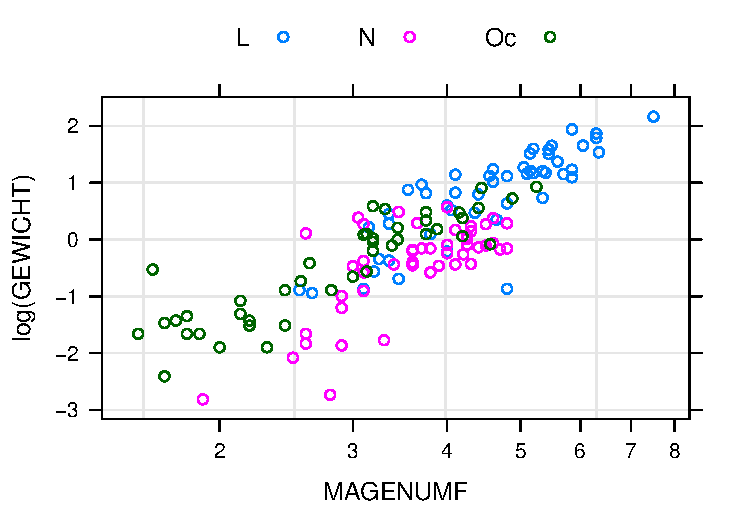
\includegraphics[width=4cm]{graphics/Bio144_2017_week3-wurmP3.pdf}
\end{center}

\alert{Categorical} and \alert{continuous} covariates were used to predict a continuous outcome (the weight of the worm).
}
\frame[containsverbatim]{

\begin{Schunk}
\begin{Sinput}
> r.lm <- lm(log(GEWICHT) ~  MAGENUMF + Gattung,d.wurm)
>  summary(r.lm)$coef
\end{Sinput}
\begin{Soutput}
              Estimate Std. Error     t value     Pr(>|t|)
(Intercept) -2.5355459 0.22147279 -11.4485663 8.617670e-22
MAGENUMF     0.7118725 0.04528843  15.7186392 1.232126e-32
GattungN    -0.5151344 0.11009219  -4.6791186 6.760621e-06
GattungOc   -0.0907298 0.12791000  -0.7093254 4.793107e-01
\end{Soutput}
\end{Schunk}

\vspace{3mm}
{\bf Remember:} What do the $p$-values ($p=0.48$ and $p<0.0001$) of the categorical covariate ``Gattung'' mean? \\[5mm]

To understand if ``Gattung'' has an effect, {\bf we need to carry out an $F$-test} (see slide 45, week 3). To this end, plot the ANOVA table:\\[2mm]
\begin{Schunk}
\begin{Sinput}
> anova(r.lm)
\end{Sinput}
\begin{Soutput}
Analysis of Variance Table

Response: log(GEWICHT)
           Df  Sum Sq Mean Sq F value    Pr(>F)    
MAGENUMF    1 104.866 104.866  409.69 < 2.2e-16 ***
Gattung     2   7.177   3.589   14.02 2.842e-06 ***
Residuals 139  35.579   0.256                      
---
Signif. codes:  0 ‘***’ 0.001 ‘**’ 0.01 ‘*’ 0.05 ‘.’ 0.1 ‘ ’ 1
\end{Soutput}
\end{Schunk}
}


\frame[containsverbatim]{\frametitle{A new example: cholesterol levels}
{\bf Example:} Cholesterol levels [mg/ml] for 30 women from two US states, Iowa and Nebraska, were measured. \\[2mm]
{\bf Question:} Do these levels differ between the states? \\[2mm]
Age (years) may be a relevant covariable. \\

\begin{center}
\setkeys{Gin}{width=0.60\textwidth}
\begin{Schunk}
\begin{Sinput}
> plot(cholesterol ~ state,data=d.chol)
\end{Sinput}
\end{Schunk}
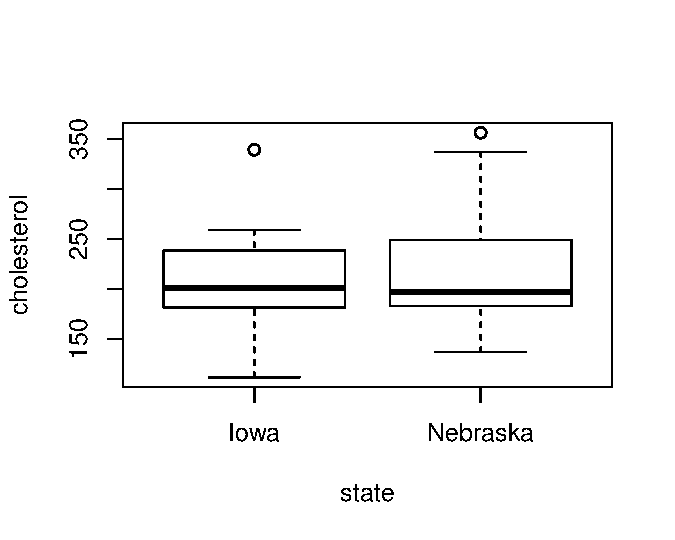
\includegraphics{Bio144_2017_week6-chol}
\end{center}
}

\frame[containsverbatim]{
The model includes state, age and the interaction of the two. The model equation is thus given as
\begin{equation*}
y_i = \beta_0 + \beta_1 (state)_i + \beta_2 (age)_i + \beta_3 (state)_i (age)_i + e_i  \ , \quad e_i \sim \N(0,\sigma_e^2) \ .
\end{equation*}
~\\

\begin{Schunk}
\begin{Sinput}
> r.aov <- aov(cholesterol ~ age*state,data=d.chol)
> summary(r.aov)
\end{Sinput}
\begin{Soutput}
            Df Sum Sq Mean Sq F value   Pr(>F)    
age          1  48976   48976  26.312 2.39e-05 ***
state        1   5456    5456   2.931   0.0988 .  
age:state    1    709     709   0.381   0.5425    
Residuals   26  48395    1861                     
---
Signif. codes:  0 ‘***’ 0.001 ‘**’ 0.01 ‘*’ 0.05 ‘.’ 0.1 ‘ ’ 1
\end{Soutput}
\end{Schunk}
\vspace{5mm}

Interpretation?
}

 
\frame[containsverbatim]{
Compare the results from the previous slide to the \texttt{lm()} output:\\[3mm]
\begin{Schunk}
\begin{Sinput}
> r.lm <- lm(cholesterol ~ age*state,data=d.chol)
> summary(r.lm)$coef
\end{Sinput}
\begin{Soutput}
                    Estimate Std. Error    t value    Pr(>|t|)
(Intercept)       35.8112138  55.116605  0.6497355 0.521562661
age                3.2381449   1.008827  3.2098104 0.003516155
stateNebraska     65.4865523  61.983368  1.0565181 0.300450053
age:stateNebraska -0.7177069   1.162845 -0.6171990 0.542471382
\end{Soutput}
\end{Schunk}
\vspace{5mm}
 
Compare the results for ``state'' also to the model without interaction:\\[3mm]
\begin{Schunk}
\begin{Sinput}
> r.lm2 <- lm(cholesterol ~ age + state,data=d.chol)
> summary(r.lm2)$coef
\end{Sinput}
\begin{Soutput}
               Estimate Std. Error  t value     Pr(>|t|)
(Intercept)   64.489772 29.3024531 2.200832 3.648161e-02
age            2.697967  0.4959532 5.439963 9.361235e-06
stateNebraska 28.651025 16.5409806 1.732124 9.466292e-02
\end{Soutput}
\end{Schunk}
~\\[2mm]
{\small {\bf Note:} the $p$-value for `state' is now the same as on the previous slide (ANOVA table).}
} 


\frame[containsverbatim]{
As always, some model checking is necessary:\\[2mm]

\setkeys{Gin}{width=0.9\textwidth}
\begin{Schunk}
\begin{Sinput}
> par(mfrow=c(1,2))
> plot(r.aov$fitted,r.aov$residuals,xlab="fitted",ylab="residuals")
> abline(h=0,lty=2)
> qqnorm(r.aov$fitted)
> qqline(r.aov$fitted)
\end{Sinput}
\end{Schunk}
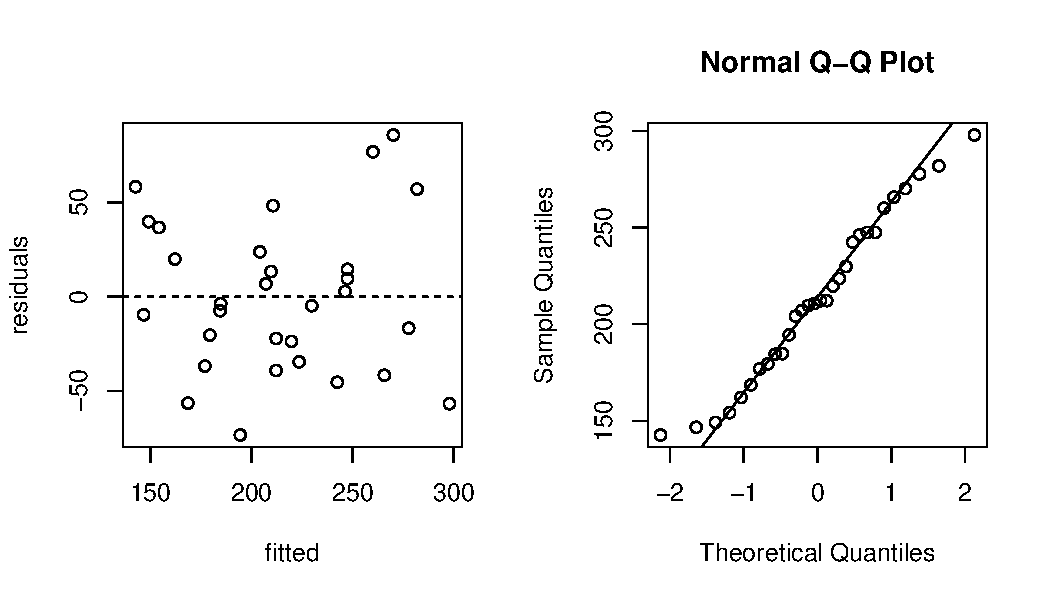
\includegraphics{Bio144_2017_week6-009}
~\\
$\rightarrow$ This seems ok.
}
 
\frame{\frametitle{A final word on ANCOVA}
ANCOVA unifies several concepts that we approached in this course so far:\\[2mm]

\begin{itemize}
\item Linear regression\\[3mm]
\item Categorical covariates\\[3mm]
\item Interactions (of continuous and categorical covariates)\\[3mm]
\item Analysis of Variance (ANOVA)\\[6mm]
\end{itemize}

As such, it is a {\bf special case of the linear model}.
} 
 
 
\frame{\frametitle{An introduction to linear Algebra}
\vspace{-2mm}
Who has some knowledge of linear Algebra?\\[4mm]

{\bf Overview}
\begin{itemize}

\item The basics about  
\begin{itemize}
\item vectors \\[1mm]
\item matrices \\[1mm]
\item matrix algebra \\[1mm]
\item matrix multiplication \\[2mm]
\end{itemize}
\item Why is linear Algebra useful? \\[2mm]
\item What does it have to do with data analysis and statistics?\\[2mm]
\item Regression equations in matrix notation.
\end{itemize}
} 
 
 
\frame{\frametitle{Motivation}
Why are vectors, matrices and their algebraic rules useful?\\[4mm]

\begin{itemize}
\item[\bf Example 1:] The observations for a covariate $\bm{x}$ or the response $\bm{y}$ for all individuals $1\leq i\leq n$ can be stored in a vector (vectors and matrices are always given in {\bf bold} letters):
\begin{equation*}
\bm{x}=\left(
\begin{array}{c}
x_1 \\
x_2 \\
... \\
x_n
\end{array}
\right) \ , \quad
\bm{y}=\left(
\begin{array}{c}
y_1 \\
y_2 \\
... \\
y_n
\end{array}
\right)  \ .
\end{equation*}
~\\[2mm]
\item[\bf Example 2:] Covariance matrices for multiple variables. Say we have $\bm{x}^{(1)}$ and $\bm{x}^{(2)}$. The \alert{covariance matrix} is then given as
\begin{equation*}
\left(
\begin{array}{cc}
\Var(\bm{x}^{(1)}) & \Cov(\bm{x}^{(1)},\bm{x}^{(2)}) \\
\Cov(\bm{x}^{(1)},\bm{x}^{(2)}) & \Var(\bm{x}^{(2)}) \\
\end{array}
\right) \ .
\end{equation*}
~\\
\end{itemize}
} 


\frame{\label{sl:examples}
\begin{itemize}
\item[\bf Example 3:] The \alert{data} (e.g.\ of some regression model) can be stored in a \alert{matrix}:
\begin{equation*}
\bm{\tilde{X}} = 
\left(
\begin{array}{ccc}
1 & x_1^{(1)} &  x_2^{(1)}\\
1 & x_2^{(1)} & x_2^{(2)} \\
... & ... &... \\
1 & x_n^{(1)} & x_n^{(2)}
\end{array}
\right) \ .
\end{equation*}
This is the so-called \alert{design matrix} with a vector of 1's in the first column.~\\[4mm]

\item[\bf Example 4:] A linear regression model can be written compactly using \alert{matrix multiplication}:
%
\begin{equation*}
\bm{y} = \bm{\tilde{X}} \cdot \bm{\tilde\beta} + \bm{e}  \ ,
\end{equation*}

with $\bm{\tilde\beta}$ the vector of regression coefficients and $\bm{\epsilon}$ the vector of residuals.
\end{itemize}
}

\frame{\frametitle{}
Why do we discuss this topic in our course?

\begin{itemize}
\item Useful for \alert{compact notation}.\\[2mm]
\item Enabels you to \alert{understand many statistical texts} (books, research articles) that remain inaccessible otherwise. \\[2mm]
\item More advanced concepts often rely on linear algebra, e.g. \alert{principal component analysis} (PCA) or \alert{random effects} models.\\[2mm]
\item Often useful for \alert{efficient coding}, e.g. in R, which helps to increase speed and to reduce error rates.\\[2mm]
\item Is part of a \alert{general education} (Allgemeinbildung) ;-) \\
\end{itemize}
}

\frame{\frametitle{Matrices}
An $n\times m$ \alert{Matrix} is given as
\begin{equation*}
\bm{A} = \left(
\begin{array}{cccc}
a_{11} & a_{12} &  ... & a_{1m}\\
a_{21} & a_{22} & ... & a_{2m} \\
\vdots & \vdots &  & \vdots \\
a_{n1} & a_{n2} & ... & a_{nm}
\end{array}\right) \ ,
\end{equation*}
with rows $1 = 1, \ldots , n$ and columns $j=1,\ldots,m$.\\[4mm]

{\bf Quadratic matrix:} $n=m$. Example:
\begin{equation*}
\left(
\begin{array}{ccc}
1 & 2 & 3 \\
4 & 3 & 2 \\
6 & 1 & 9 \\
\end{array}
\right)
\end{equation*}
}

\frame{\frametitle{}
{\bf Symmetric matrix:} $a_{ij} = a_{ji}$. Example:
\begin{equation*}
\left(
\begin{array}{ccc}
1 & 2 & 3 \\
2 & 3 & 4 \\
3 & 4 & 5 \\
\end{array}
\right) \ .
\end{equation*}
~\\[2mm]

{\bf The diagonal of a quadratic matrix} is given by $(a_{11},a_{22},\ldots , a_{nn})$. Example: the diagonal of the above matrix is given as
\begin{equation*}
(a_{11},a_{22},a_{33}) = (1,3,5) \ .
\end{equation*}
~\\[2mm]

{\bf Diagonal matrix:} A matrix that has entries $\neq 0$ \alert{only on the diagonal}. Example:
\begin{equation*}
\left(
\begin{array}{ccc}
1 & 0 & 0 \\
0 & 3 & 0 \\
0 & 0 & 5 \\
\end{array}
\right) \ .
\end{equation*}

}

\frame{\frametitle{}
{\bf Transposing a matrix:} Given a matrix $\bm{A}$. Exchange the rows by the columns and vice versa. This leads to the \alert{transposed matrix} $\bm{A}^\top$:
\begin{equation*}
\bm{A} = \left(
\begin{array}{cccc}
a_{11} & a_{12} &  ... & a_{1m}\\
a_{21} & a_{22} & ... & a_{2m} \\
\vdots & \vdots &  & \vdots \\
a_{n1} & a_{n2} & ... & a_{nm}
\end{array}\right) \quad \Rightarrow \quad
\bm{A}^\top = \left(
\begin{array}{cccc}
a_{11} & a_{21} &  ... & a_{m1}\\
a_{12} & a_{22} & ... & a_{m2} \\
\vdots & \vdots &  & \vdots \\
a_{1n} & a_{2n} & ... & a_{mn}
\end{array}\right) \ .
\end{equation*}
~\\[2mm]

Examples (note also the change of dimensions):
\begin{equation*}
\bm{A} = \left(
\begin{array}{cccc}
1 & 2 & 3 & 4\\
5 & 6 & 7 & 8 \\
9 & 10  & 11  & 12 \\
13 & 14 & 15 & 16 \\
\end{array}\right) \quad \Rightarrow \quad 
\bm{A}^\top = \left(
\begin{array}{cccc}
1 & 5 & 9 & 13\\
2 & 6 & 10 & 14 \\
3 & 7  & 11  & 15 \\
4 & 8 & 12 & 16\\
\end{array}\right)
\end{equation*}

\begin{equation*}
\bm{A} = \left(
\begin{array}{cccc}
1 & 2 & 3 & 4\\
5 & 6 & 7 & 8 \\
\end{array}\right) \quad \Rightarrow \quad 
\bm{A}^\top = \left(
\begin{array}{cc}
1 & 5  \\
2 & 6   \\
3 & 7  \\
4 & 8 \\
\end{array}\right)
\end{equation*}
}

\frame{

\begin{itemize}
\item Transposing a matrix \alert{twice} leads to the original matrix: $$(\bm{A}^\top)^\top = \bm{A} \ .$$ 
~\\[2mm]

\item When a matrix is \alert{symmetric}, then $$\bm{A}^\top = \bm{A} \ .$$
This is true in particular for diagonal matrices.
\end{itemize}
}

\frame{\frametitle{Vectors}
A vector is nothing else than $n$ numbers written in a column:
\begin{equation*}
\bm{b} = \left(
\begin{array}{c}
b_1 \\ 
b_2 \\
\vdots \\
b_n
\end{array}
\right)
\end{equation*}
~\\[2mm]

{\bf Transposing} a vector leads to a \emph{row vector}:
\begin{equation*}
\left(
\begin{array}{c}
b_1 \\ 
b_2 \\
\vdots \\
b_n
\end{array}
\right)^\top
 = \left(
\begin{array}{cccc}
b_1  & b_2  & \hdots & b_n
\end{array}
\right)
\end{equation*}

{\bf Note:} By definition (by default), a vector is always a column vector. 
}

\frame{\frametitle{Addition and substraction}
\begin{itemize}
\item Adding and substracting matrices and vectors is only possible when the objects have the \alert{same dimension}.
\item Examples: Elementwise addition (or substraction)

\begin{equation*}
\left(
\begin{array}{ccc}
1 & 2 & 3 \\ 
4 & 5 & 6 \\
\end{array}
\right) 
+
\left(
\begin{array}{ccc}
3 & 2 & 1 \\ 
6 & 5 & 4 \\
\end{array}
\right) 
 = 
 \left(
\begin{array}{ccc}
4 & 4 & 4 \\ 
10 & 10 & 10 \\
\end{array}
\right)
\end{equation*}

\begin{equation*}
\left(
\begin{array}{c}
1   \\ 
4  \\
\end{array}
\right) 
-
\left(
\begin{array}{ccc}
3   \\ 
9 \\
\end{array}
\right) 
 = 
 \left(
\begin{array}{c }
-2\\ 
-5\\
\end{array}
\right)
\end{equation*}


~\\[2mm]

\item But this addition is \alert{not defined}:
\begin{equation*}
\left(
\begin{array}{ccc}
1 & 2 & 3 \\ 
4 & 5 & 6 \\
\end{array}
\right) 
+
\left(
\begin{array}{cc}
3 & 6   \\ 
2 & 5  \\
1 & 4
\end{array}
\right)  = 
\end{equation*}

\end{itemize}
}


\frame{\frametitle{Multiplication by a scalar}
Multiplication with a ``number'' (scalar) is simple: Multiply each element in a vector or a matrix.\\[2mm]

Examples:


\begin{equation*}
3 \cdot \left(
\begin{array}{ccc}
1 & 2 & 3 \\ 
4 & 5 & 6 \\
\end{array}
\right) 
 = 
 \left(
\begin{array}{ccc}
3 & 6 & 9 \\ 
12 & 15 & 18 \\
\end{array}
\right)
\end{equation*}


\begin{equation*}
-2 \cdot \left(
\begin{array}{c}
1 \\ 
4 \\
-2 \\
\end{array}
\right) 
 = 
 \left(
\begin{array}{c}
-2 \\ 
-8 \\
4 \\
\end{array}
\right) 
\end{equation*}
}

\frame{\frametitle{Matrix multiplication}

\colorbox{lightgray}{\begin{minipage}{10cm}
The multiplication of two matrices $\bm{A}$ and $\bm{B}$ is \alert{defined if}\\[2mm]
Number of columns in $\bm{A}$ = Number of rows in $\bm{B}$.
\end{minipage}}
~\\[2mm]

It is easiest to explain matrix multiplication with an example:
\begin{eqnarray*}
\left(
\begin{array}{cc}
2 & 1 \\
-1 & 0 \\
3 & 1 \\
\end{array}
\right) \cdot 
\left(
\begin{array}{cc}
3 & 1 \\
4 & -2 \\
\end{array}
\right) &=& 
\left(
\begin{array}{cc}
2\cdot 3 + 1\cdot 4   &   2\cdot 1 + 1\cdot (-2) \\
(-1)\cdot 3 + 0\cdot 4 & (-1)\cdot 1 + 0\cdot (-2) \\
3\cdot 3 + 1\cdot 4 & 3\cdot 1 + 1\cdot (-2)
\end{array}
\right) \\
&=& \left(
\begin{array}{cc}
10   &   0 \\
-3  & -1 \\
13  & 1
\end{array}
\right)
\end{eqnarray*} 

\href{http://matrix.reshish.com/multiplication.php}
{\beamergotobutton{Matrix multiplication app}}
}

\frame[allowframebreaks]{\frametitle{Matrix multiplication rules}
Attention: Matrix multiplication does \alert{not} follow the same rules as scalar multiplication!!!\\[2mm]

\begin{itemize}
\item It can happen that $\bm{A}\cdot \bm{B}$ can be calculated, but $\bm{B}\cdot \bm{A}$ is not defined (see example on previous slide). \\[4mm]
\item In general: $\bm{A}\cdot \bm{B} \neq  \bm{B}\cdot \bm{A}$, even if both are defined.\\[4mm]
\item It can happen that $\bm{A}\cdot \bm{B} =\bm{0}$ ($\bm{0}$ matrix), although both $\bm{A}\neq \bm{0}$ and $\bm{B}\neq \bm{0}$. \\[4mm]
\item The \alert{Assoziativgesetz holds:} $\bm{A}\cdot (\bm{B} \cdot \bm{C}) = (\bm{A}\cdot \bm{B}) \cdot \bm{C}$. \\[4mm]
\item The \alert{Distributivgesetz holds:} 
\begin{eqnarray*}
\bm{A}\cdot (\bm{B} + \bm{C}) &=& \bm{A}\cdot \bm{B} +   \bm{A}\cdot \bm{C}  \\
(\bm{A} + \bm{B} ) \cdot \bm{C}) &=& \bm{A}\cdot \bm{C} +   \bm{B}\cdot \bm{C} 
\end{eqnarray*}
\item Transposing inverts the order: $(\bm{A}\cdot \bm{B})^\top = \bm{B}^\top \cdot \bm{A}^\top$.\\[4mm]
\item The product $\bm{A}\cdot\bm{A}^\top$ is \alert{always symmetric}. \\[4mm]
\item All these rules also hold for \alert{vectors}, which can be interpreted as $n\times 1$ matrices:
\begin{equation*}
\bm{a}\cdot \bm{b}^\top = 
\left(
\begin{array}{cccc}
a_1b_1 & a_1 b_2 & \ldots & a_1 b_m \\
a_2b_1 & a_2 b_2 & \ldots & a_2 b_m \\
\vdots & \vdots & & \vdots \\
a_n b_1 & a_n b_2 & \ldots & a_n b_m \\
\end{array}
\right)
\end{equation*}
If $\bm{a}$ and $\bm{b}$ have the \alert{same length}:
\begin{equation*}
\bm{a}^\top \cdot \bm{b}  = 
 \sum_i a_i  b_i
\end{equation*}
\end{itemize}
}


\frame{\frametitle{Short exercises}
Given vectors $\bm{a}$ and $\bm{b}$ and matrix $\bm{C}$:
\begin{equation*}
\bm{a} =\left( \begin{array}{c} 1 \\  -2 \\ 3 \\ 0 \end{array}\right), \quad
\bm{b} = \left( \begin{array}{c}-2\\  4 \end{array}\right), \quad 
\bm{C}=\left(\begin{array}{cc} 1 & 0 \\ -1 & 2 \end{array}\right)
\end{equation*}
~\\[4mm]

Calculate, if defined
\begin{itemize}
\item $\bm{a}^\top \cdot \bm{b}$ \\[2mm]
\item $\bm{a} \cdot \bm{b}^\top$ \\[2mm]
\item $\bm{C}\cdot \bm{a}$ \\[2mm]
\item $\bm{C}\cdot \bm{b}$ \\[2mm]
\end{itemize}
}


\frame{\frametitle{The length of a vector}
The \alert{length of a vector} $\bm{a}^\top=(a_1,a_2,\ldots, a_n)$ is defined as $||\bm{a}||$ with
\begin{equation*}
||\bm{a}||^2 = \bm{a}^\top \cdot \bm{a} =   \sum_i a_i^2  \ .
\end{equation*}

This is basically the \alert{Pythagoras} idea in 2, 3, ... $n$ dimensions.\\[4mm]

In 2 dimensions: $||\bm{a}||^2 = a_1^2 + a_2^2$:

\begin{center}
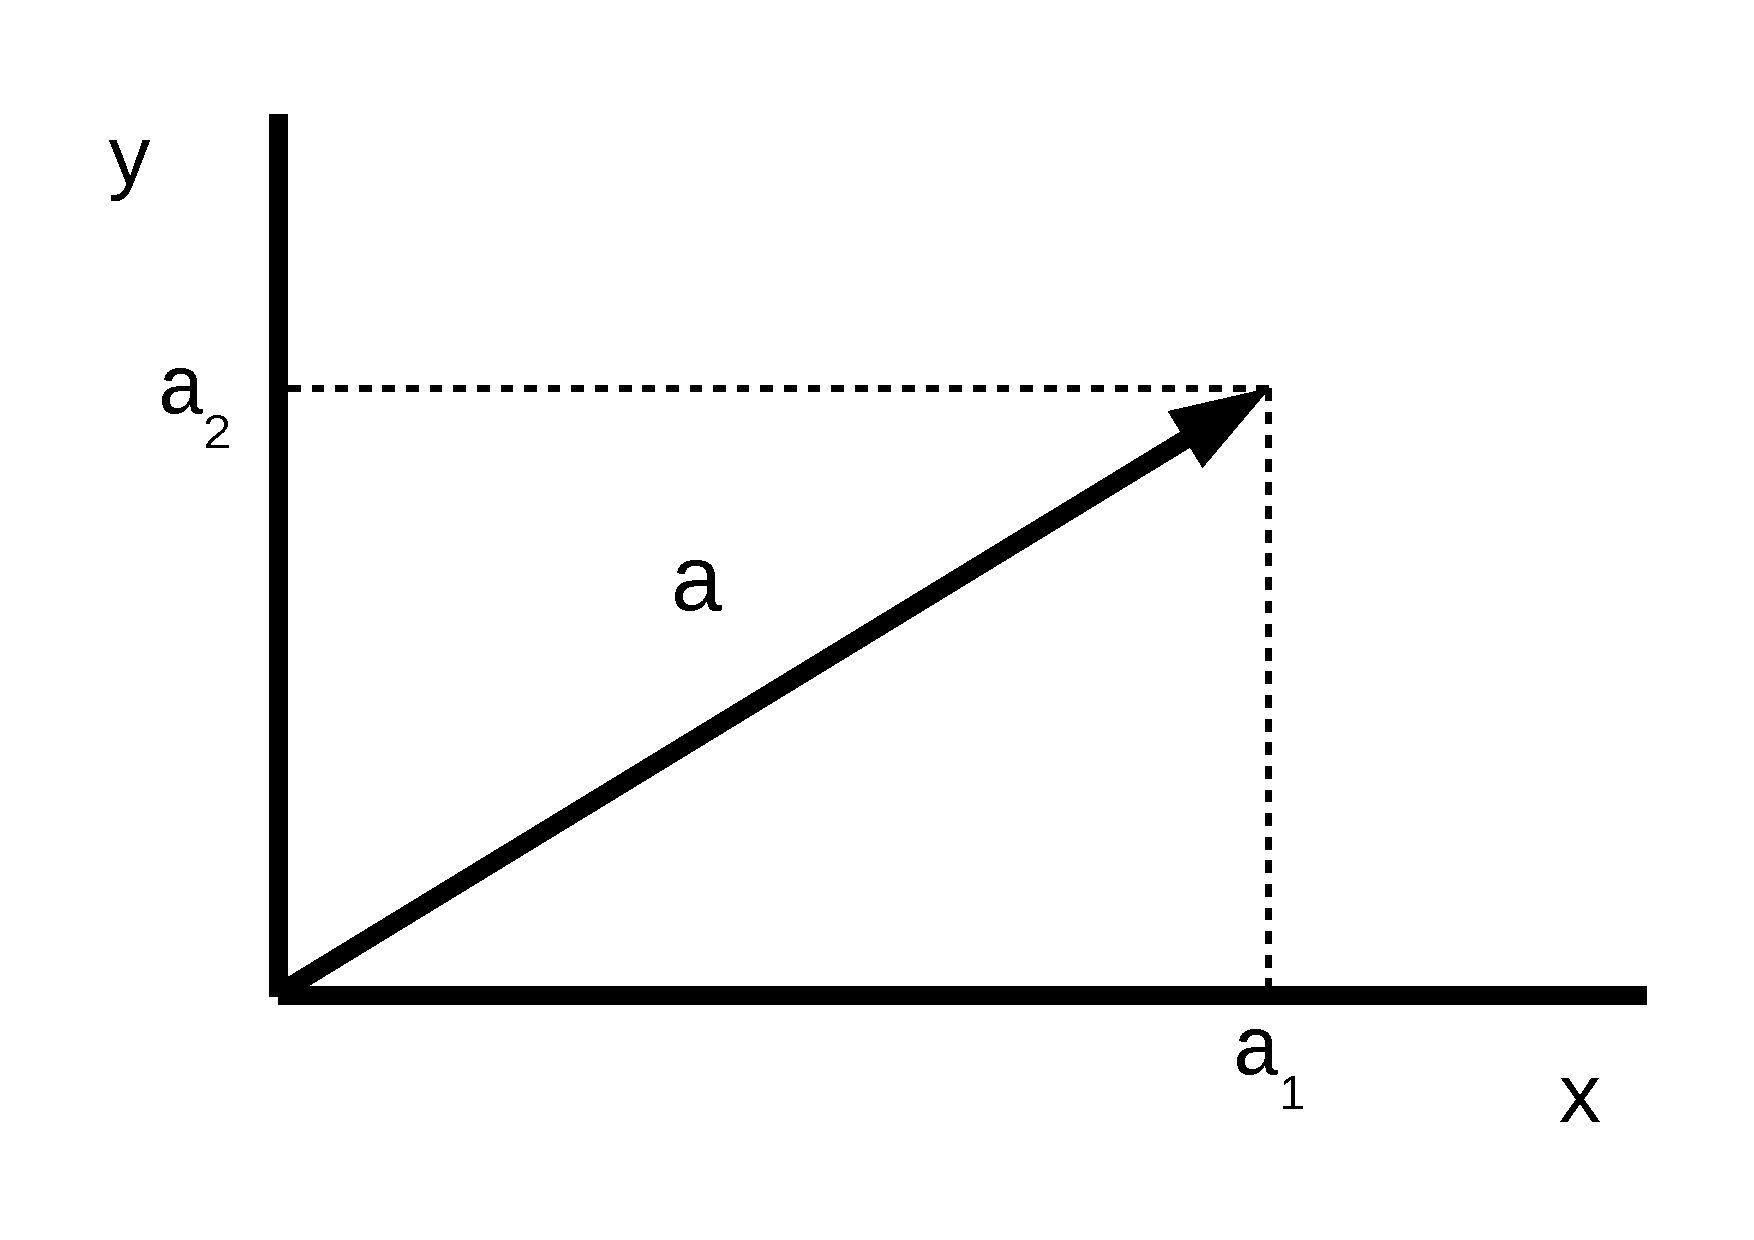
\includegraphics[width=4cm]{graphics/pythagoras.pdf}
\end{center}
}


\frame{\frametitle{Identity matrix (Einheitsmatrix)}
The identity matrix (of dimension $m$) is probably the simples matrix that exists. It has 1's on the diagonal and 0's everywhere else:

\begin{equation*}
\bm{I} = 
\left( 
\begin{array}{cccc}
1 & 0 & \ldots & 0 \\
0 & 1 & \ldots & 0 \\
\vdots & \vdots && \vdots \\
0 & 0 & \ldots & 1 
\end{array}
\right)
\end{equation*}
~\\[2mm]

Multiplication with the identity matrix leaves a $m\times n$ matrix $\bm{A}$ unchanged:\\
$$\bm{I} \cdot \bm{A} = \bm{A} \cdot \bm{I} = \bm{A} \ .$$
}

\frame{\frametitle{Inverse matrix}
\colorbox{lightgray}{\begin{minipage}{10cm}
Given a quadratic matrix $\bm{A}$ that fulfills
\begin{equation*}
\bm{B}\cdot \bm{A} = \bm{I} \ ,
\end{equation*}
then $\bm{B}$ is called the \alert{inverse} of $\bm{A}$ (and vice versa). One then writes 
$$\bm{B}=\bm{A}^{-1} \ .$$
\end{minipage}}
~\\[2mm]

Note: 
\begin{itemize}
\item In that case it also holds that $\bm{A}\cdot \bm{B} = \bm{I}$.\\[2mm]
\item Therefore: $\, \bm{A}=\bm{B}^{-1} \quad  \Leftrightarrow \quad  \bm{B}=\bm{A}^{-1}$ \\
\end{itemize}

}

\frame{
\begin{itemize}
\item The inverse of $\bm{A}$ may \alert{not exist}. If it exists, $\bm{A}$ is \alert{regular}, otherwise \alert{singular}.\\[4mm]
\item $(\bm{A}^{-1})^{-1} = \bm{A}$. \\[4mm]
\item The inverse of a matrix product is given as 
$$(\bm{A}\cdot \bm{B})^{-1} = \bm{B}^{-1} \cdot \bm{A}^{-1} \ .$$\\

\item It is
$$(\bm{A}^\top)^{-1} = (\bm{A}^{-1})^\top \ .$$
Therefore one may also write $\bm{A}^{-\top}$.
\end{itemize}

}

\frame{\frametitle{Linear equation system in matrix notation}
Remember example 4 from slide \ref{sl:examples}: We said that a linear regression model can be written compactly using \alert{matrix multiplication}:
%
\begin{equation*}
\bm{y} = \bm{\tilde{X}} \cdot \bm{\tilde\beta} + \bm{e}  \ .
\end{equation*}
~\\[2mm]

Task: Verify this now, using a model with two variables $\bm{x}^{(1)}$ and $\bm{x}^{(2)}$ and
\begin{equation*}
\bm{y}=\left(\begin{array}{c} y_1 \\ y_2 \\ \vdots \\ y_n\end{array}\right), \;
\, \bm{\tilde\beta}=\left(\begin{array}{c} \beta_0 \\ \beta_1 \\ \beta_2\end{array}\right), \;
\bm{\tilde{X}} = 
\left(
\begin{array}{ccc}
1 & x_1^{(1)} &  x_2^{(1)}\\
1 & x_2^{(1)} & x_2^{(2)} \\
... & ... &... \\
1 & x_n^{(1)} & x_n^{(2)}
\end{array}
\right), \;
\bm{e}=\left(\begin{array}{c} e_1 \\ e_2 \\ \vdots \\ e_n\end{array}\right).
\end{equation*}
}


\frame{\frametitle{}
It can be shown (see Stahel 3.4f,g) that \alert{the least-squares estimates} $\hat{\bm\beta}$ can be calculated as
\begin{equation*}
\hat{\bm\beta} = (\tilde{\bm{X}}^\top \tilde{\bm{X}})^{-1} \cdot \tilde{\bm{X}}^\top \cdot \bm{y} 
\end{equation*}
~\\[4mm]
Does this look complicated? \\[4mm]
Let's test this in R ....
}


\frame[containsverbatim]{\frametitle{Doing linear algebra in R}
Let us look at model $\bm{y} = \bm{\tilde{X}} \cdot \bm{\tilde\beta} + \bm{e}$ with coefficients $\beta_0=10, \beta_1=5, \beta_2=-2$ and variables\\

\begin{center}
\begin{tabular}{ccc}
$i$ & $x_i^{(1)}$ & $x_i^{(2)}$ \\
\hline
1 & 0 & 4 \\
2 & 1 & 1\\
3 & 2 & 0\\
4 & 3 &1\\
5 & 4 & 4\\
\end{tabular}
\end{center}

Thus the model is given as 
\begin{equation*}
y_i = 10 + 5 x_i^{(1)} + -2 x_i^{(2)} + e_i \ , \text{for }\quad 1\leq i \leq n \ . 
\end{equation*}
Let us start by generating the ``true'' response, calculated as $\bm{\tilde{X}} \bm{\tilde\beta}$:\\[2mm]
}

\frame[containsverbatim]{
\begin{Schunk}
\begin{Sinput}
> x1 <- c(0,1,2,3,4)
> x2 <- c(4,1,0,1,4)
> Xtilde <- matrix(c(rep(1,5),x1,x2),ncol=3)
> Xtilde
\end{Sinput}
\begin{Soutput}
     [,1] [,2] [,3]
[1,]    1    0    4
[2,]    1    1    1
[3,]    1    2    0
[4,]    1    3    1
[5,]    1    4    4
\end{Soutput}
\begin{Sinput}
> beta <- c(10,5,-2)
> t.y <- Xtilde%*%beta
> t.y
\end{Sinput}
\begin{Soutput}
     [,1]
[1,]    2
[2,]   13
[3,]   20
[4,]   23
[5,]   22
\end{Soutput}
\end{Schunk}
~\\[2mm]

Matrix multiplication in R is done by the \alert{\texttt{\%*\%}} symbol. 
 }

\frame[containsverbatim]{
Next, we generate the vector containing the $e_i \sim \N(0,\sigma_e^2)$ with $\sigma_e^2=1$:\\[2mm]

\begin{Schunk}
\begin{Sinput}
> e <- runif(5,0,1)
\end{Sinput}
\end{Schunk}

~\\[2mm]
which we add to the ``true'' $\bm{y}=\bm{\tilde{X}} \bm{\tilde\beta}$ values, to obtain the ``observed'' values:\\[2mm]
\begin{Schunk}
\begin{Sinput}
> t.Y <- t.y  + e
\end{Sinput}
\end{Schunk}

~\\[2mm]
It is now possible to fit the model with \texttt{lm}:\\[2mm]
\begin{Schunk}
\begin{Sinput}
> r.lm <- lm(t.Y ~ x1 + x2)
> summary(r.lm)$coef
\end{Sinput}
\begin{Soutput}
             Estimate Std. Error   t value     Pr(>|t|)
(Intercept) 10.559927 0.15368505  68.71148 0.0002117402
x1           4.892453 0.05163983  94.74186 0.0001113893
x2          -1.948033 0.04364362 -44.63500 0.0005015590
\end{Soutput}
\end{Schunk}

}


\frame[containsverbatim]{
Alternatively, we can use formula

\begin{equation*}
\hat{\bm\beta} = (\tilde{\bm{X}}^\top \tilde{\bm{X}})^{-1}   \tilde{\bm{X}}^\top   \bm{y} 
\end{equation*}

to find the parameter estimates:\\[2mm]

\begin{Schunk}
\begin{Sinput}
> solve(t(Xtilde) %*% Xtilde)  %*%  t(Xtilde) %*% t.Y
\end{Sinput}
\begin{Soutput}
          [,1]
[1,] 10.559927
[2,]  4.892453
[3,] -1.948033
\end{Soutput}
\end{Schunk}
~\\[2mm]

\begin{itemize}
\item \texttt{solve()} calculates the \alert{inverse}.
\item \texttt{t()} gives the \alert{transposed}.\\[4mm]
\end{itemize}

{\bf Task:} Do this calculation by yourself and verify for each step that the dimensions of the matrices and the vector are indeed fitting, so that this expression is defined.
}

\frame{\frametitle{Some R commands for matrix algebra}
Ev?}

\frame{\frametitle{Distribution of the $\bm{\beta}$ coefficients}
See chapter 3.5 in Stahel: Linear algebra is useful to find the actual distribution of the regression coefficients $\bm\beta$.\\[4mm]

No need to know this by heart -- but please remember:\\[2mm]

\colorbox{lightgray}{\begin{minipage}{10cm}
Finding the joint distribution for $\bm\beta$ is {\bf much harder} without linear alebra.
\end{minipage}}
}



\frame{\frametitle{Summary}

}
% \frame{References:
% \bibliographystyle{Chicago}
% \bibliography{refs}
% }



\end{document}
